
\section{Preliminaries}
\label{sec:Preliminaries}
This paper designs Survivable embedded Virtual Network algorithm based on the node fault graph theorem. This section introduces the
preliminaries on the theorem.

For simplicity, we firstly introduce some notations and definitions about graph's fault tolerant in order to describe our proposed SeVN problem clearly.

\subsection{Node Fault Graph}
\subsubsection{Node Fault tolerant (NFT)}
We refer to the concept of $k$-NFT\cite{harary1996node}. Let $G(V,E)$ be a graph with $n$ nodes and $q$ edges. An $(n+k)$-node graph $G^*$ is k-node fault-tolerant, or $k$-NFT, with respect to $G$ if every graph $G^*-R$ obtained by removing any nodes set $R$ of $k>0$ nodes from $G^*$ contains $G$. Generally speaking, $G$ is subgraph isomorphism of $G^*-R$. We will refer to $G^*$ as a $k$-NFT supergraphs of $G$ or simply as a $k$-NFT($G$). We also say $G^*\cong$ $k$-NFT($G$), the set of all k-NFT($G$) supergraphs of $G$.

The complete graph $K_{n+k}$ of $n + k$ nodes is trivially a k-NFT supergraph of every $G$ that contains up to n nodes. We are concerned mainly with $k$-NFT graphs that satisfy the following optimality criterion: If $G^*$ has the smallest number $|E(G^*)|$ of edges among all $(n + k)$-node supergraphs that are $k$-NFT with respect to $G$, then $G^*$ is optimally $k$-NFT with respect to $G$. The number $NFT_{ec}$$(G,k)$ =$|E(G^*)-E(G)|$ is called the $k$-NFT edge cost of $G$. The number $NFT_{nc}$$(G,k)$ =$|V(G^*)-V(G)|$ is called the $k$-NFT node cost of $G$, however $NFT_{nc}$$(G,k)$ = k with respect with k node fault tolerant graph of graph $G$ . For example, $NFT_{nc}$$(C_5,1)$ and $NFT_{ec}$$(C_5,1)$ of graph $C_5$ is 1 and 5 respectively as demonstrated in Fig.\ref{fig:NFTexample}. Furthermore, deriving optimal graphs $G^o$ with minimal links for any general graph G has exponential complexity. To the best of the authors’ knowledge, optimal solutions are found only on regular graphs such as lines, square-grids, circles, and trees.

\begin{figure}
  \centering 
  % Requires \usepackage{graphicx}
  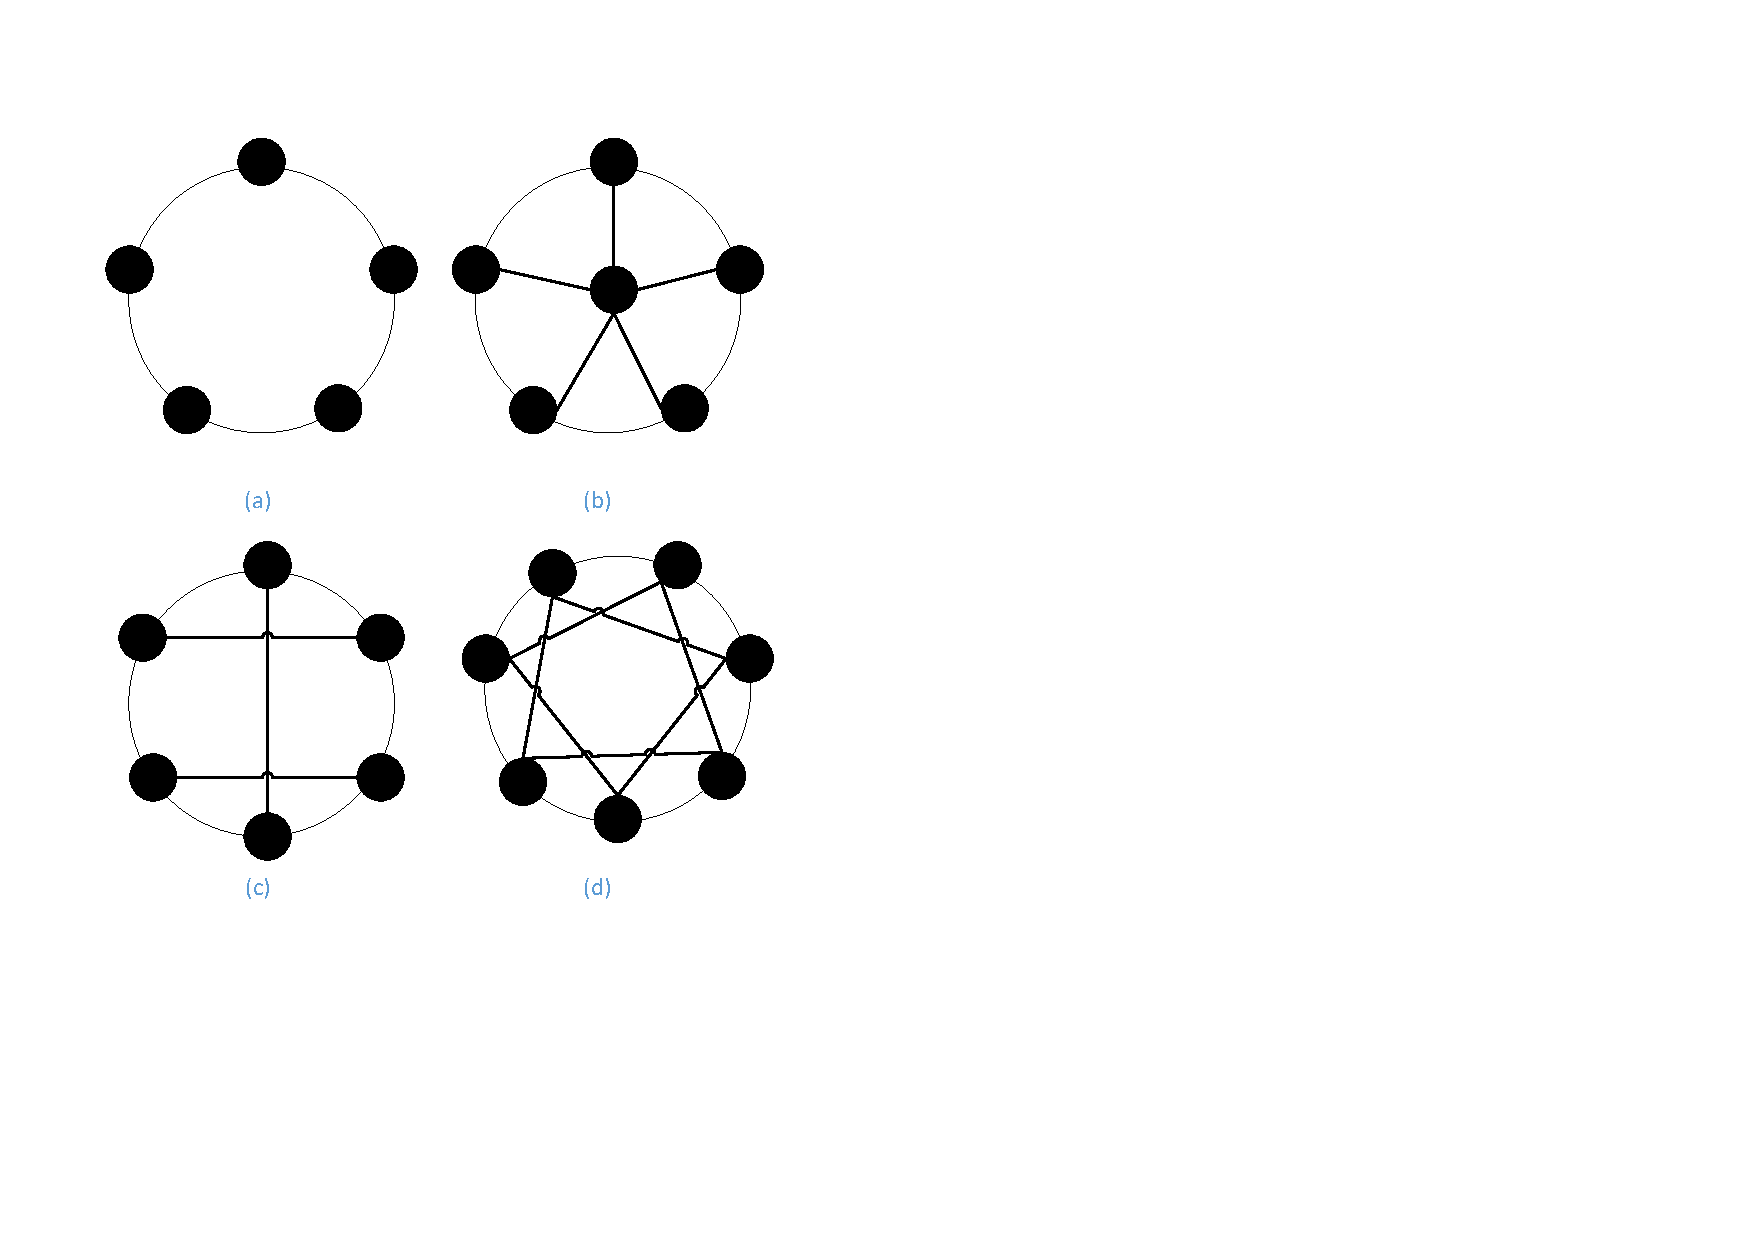
\includegraphics[width=2.5in]{Fig/NFTexample}\\
  \caption{(a)The cycle $C_5$; (b)a non-optimal $1$-NFT($C_5$), $|R|$=1 ; (c) an optimal $1$-NFT($C_5$), $|R|$=1; (d) an optimal $2$-NFT($C_5$), $|R|$=2. }\label{fig:NFTexample}
\end{figure}

\subsubsection{Function Node Fault Tolerant (FNFT)}
When every nodes of graph $G(V,E,S)$ have a specific functions set $S$ (corresponding to node's function function set) and every nodes is marked by only one function type (every node of virtual network just run only one type of function function), which is denoted by node function. A $(n+k)$-node graph $G^o$ is k-function node fault tolerant, or $k$-FNFT, with respect to $G(V,E,S)$ if every graph $G^o-R$ obtained by removing any nodes set $R$ of $k>0$ nodes from $G^o$ contains $G$, $G$ is subgraph isomorphism of $G^o-R$ and the node function of any nodes $n$ of $G$ belong function set of node $n^o$ corresponding to node $n$. We will refer to $G^o$ as a $k$-FNFT supergraphs of $G$ or simply as a $k$-FNFT($G$). The number $SNFT_{nc}$$(G,k)$ =$|V(G^o)-V(G)|$ is called the $k$-FNFT node cost of $G$. The number $SNFT_{ec}$$(G,k)$ =$|E(G^o)-E(G)|$ is called the $k$-FNFT edge cost of $G$. Suppose every node of added nodes contain all function types in current above definition.
\subsubsection{FNFT with B}
After our simple inference, if we refer the node cost $FNFT_{nc}(G,k)$  is more important cost than $FNFT_{ec}(G,k)$  edge cost, moreover the added node $B(V,S)$ could have a function set rather than contain all types of function (every node of substrate network contain various combinations of function type), Based real situation that the added node should be limited in specific function set through our analyzing the real-world practical phenomenon.(should cite a paper).
 As shown in Fig
%A backup (redundant) node b must not be able to assume full execution of a failed critical node c.

Suppose added nodes as backup node set $B(V,S)$, where every nodes of backup node set $B$ have a function set. The $k$-FNFT($G,B$) is denoted by requesting a k function node fault tolerant graph of graph $G$ and added nodes belong backup nodes set $B$. For example, as shown in Fig.\ref{fig:SNFTBexample}, every backup node have individual function set. In Fig.\ref{fig:SNFToptimal_n1Fail} displaying the transformed graph after node $v_1$ failure.

%The limited node of $G^o-G$ with respect to any $G^o$ is used as inserted node from specific node set $B$ which is premise. k-specific node fault-tolerant graph of $G$ with limit-inserted node set $B$ is denoted by k-FNFT($G,B$).


\begin{figure*}[tp]
\centering
\begin{minipage}[t]{0.3\linewidth}
\centering
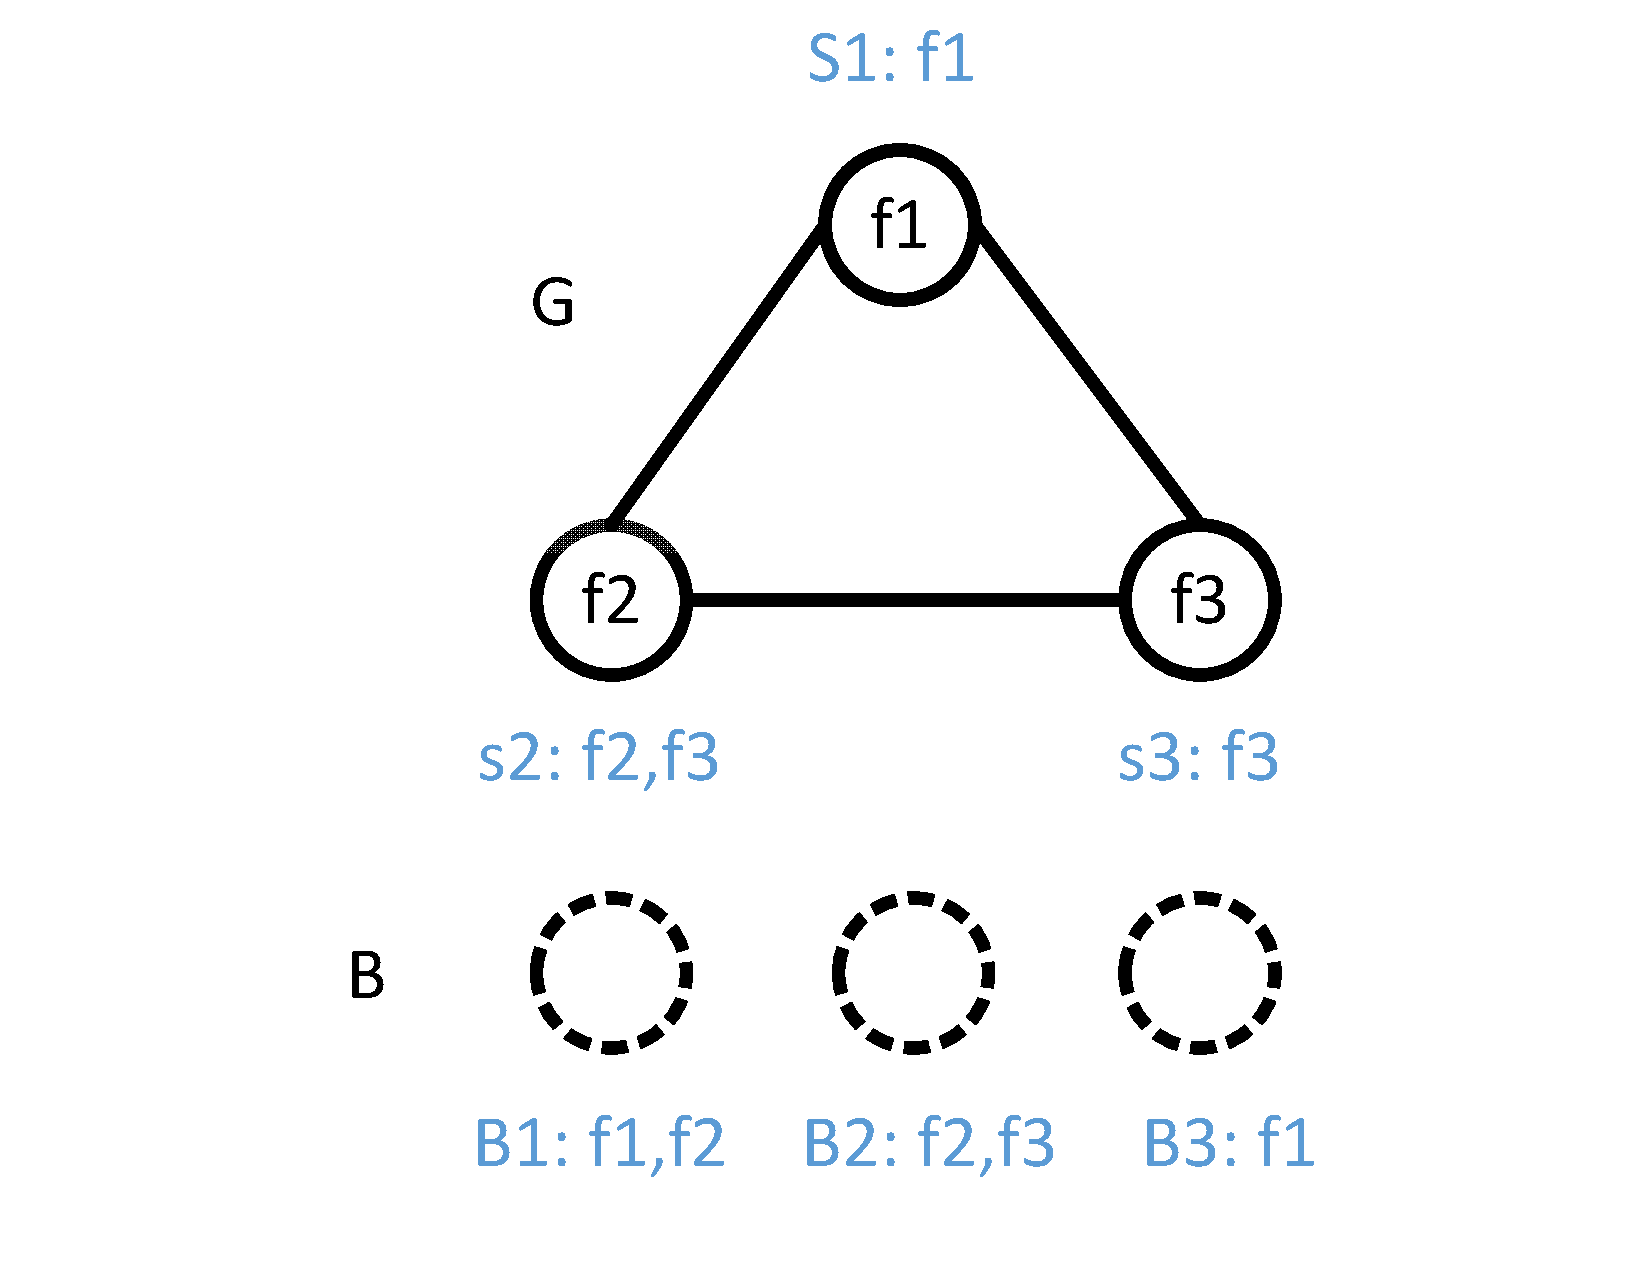
\includegraphics[width=1.5in]{Fig/SNFTBexample}\\
\caption{Graph $G(V,E,S)$: V=$\{v_1,v_2,v_3\}$, E=$\{v_1v_2,v_2v_3,v_3v_1\}$, S=$\{\{s_1\},\{s_2,s_3\},\{s_3\}\}$. Backup node $B(V,S)$: V=$\{b_1,b_2,b_3\}$, S=$\{\{s_1,s_2\},\{s_2,s_3\},\{s_1\}\}$ }\label{fig:SNFTBexample}
\end{minipage}
\hfill
\begin{minipage}[t]{0.3\linewidth}
\centering
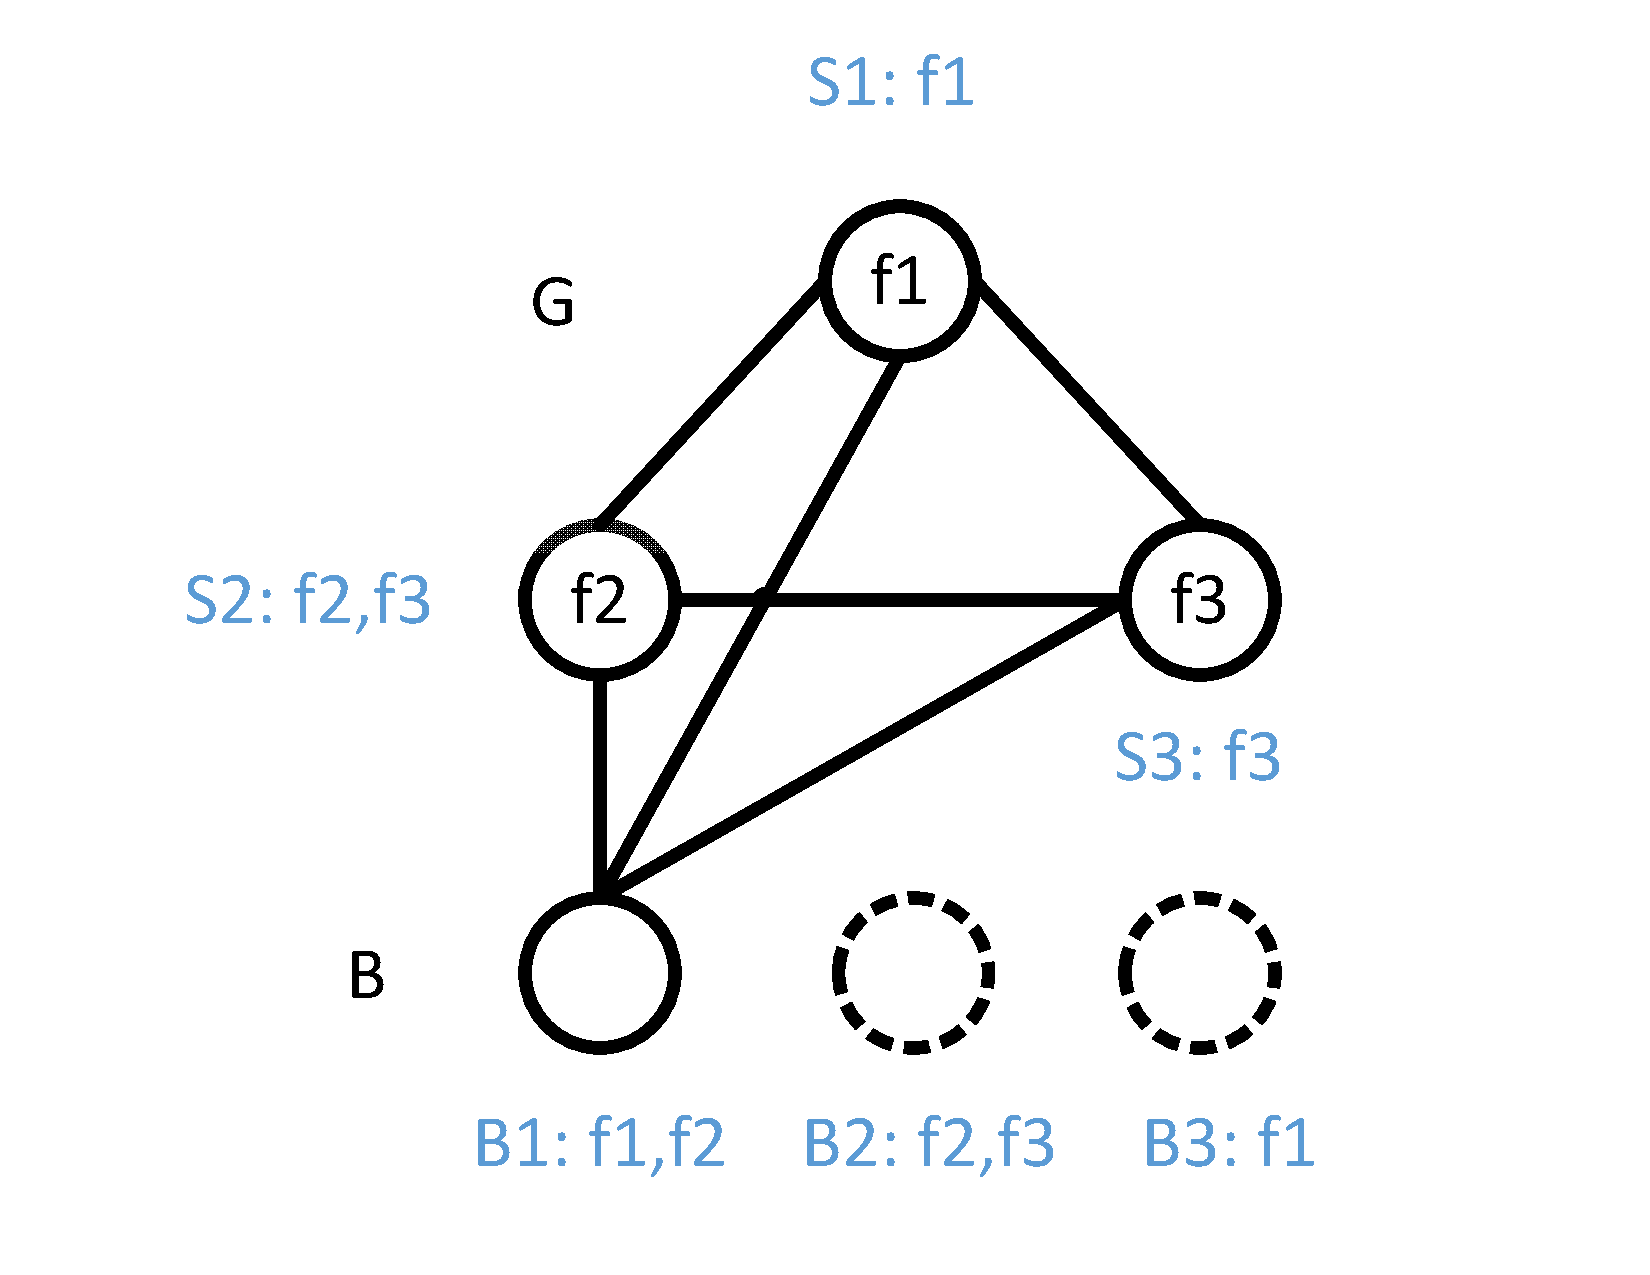
\includegraphics[width=1.5in]{Fig/SNFToptimal}\\
\caption{optimal $1$-FNFT($G(V,E,S),B(V,S)$), $SNFT_{nc}$$(G,1,B)$=1, $SNFT_{ec}$$(G,1,B)$=3.}\label{fig:SNFToptimal}
\end{minipage}
\hfill
\begin{minipage}[t]{0.3\linewidth}
\centering
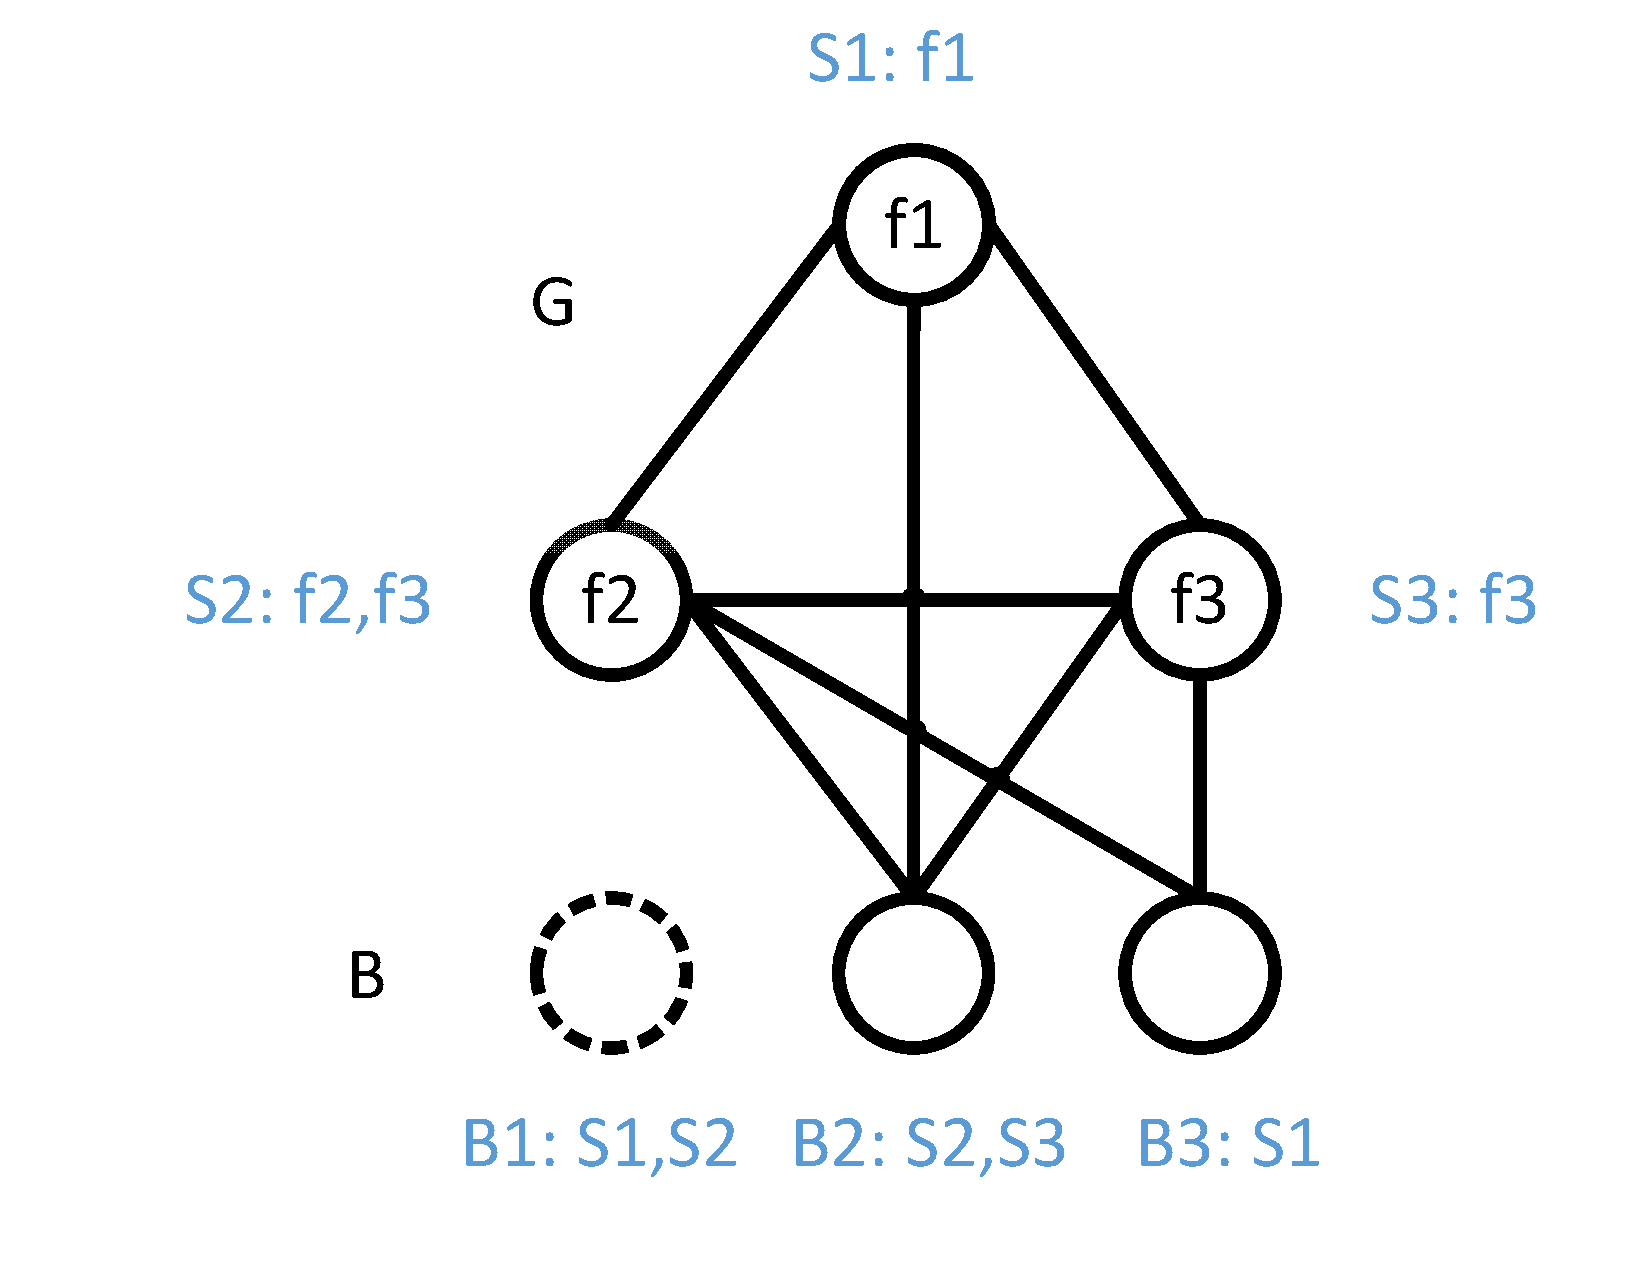
\includegraphics[width=1.5in]{Fig/SNFTnonoptimal}\\
\caption{non optimal $k$-FNFT($G(V,E,S),B(V,S)$), $SNFT_{nc}$$(G,1,B)$=2, $SNFT_{ec}$$(G,1,B)$=5}\label{fig:SNFTnonoptimal}
\end{minipage}
\end{figure*}


\begin{figure*}[tp]
\centering
\begin{minipage}[t]{0.3\linewidth}
\centering
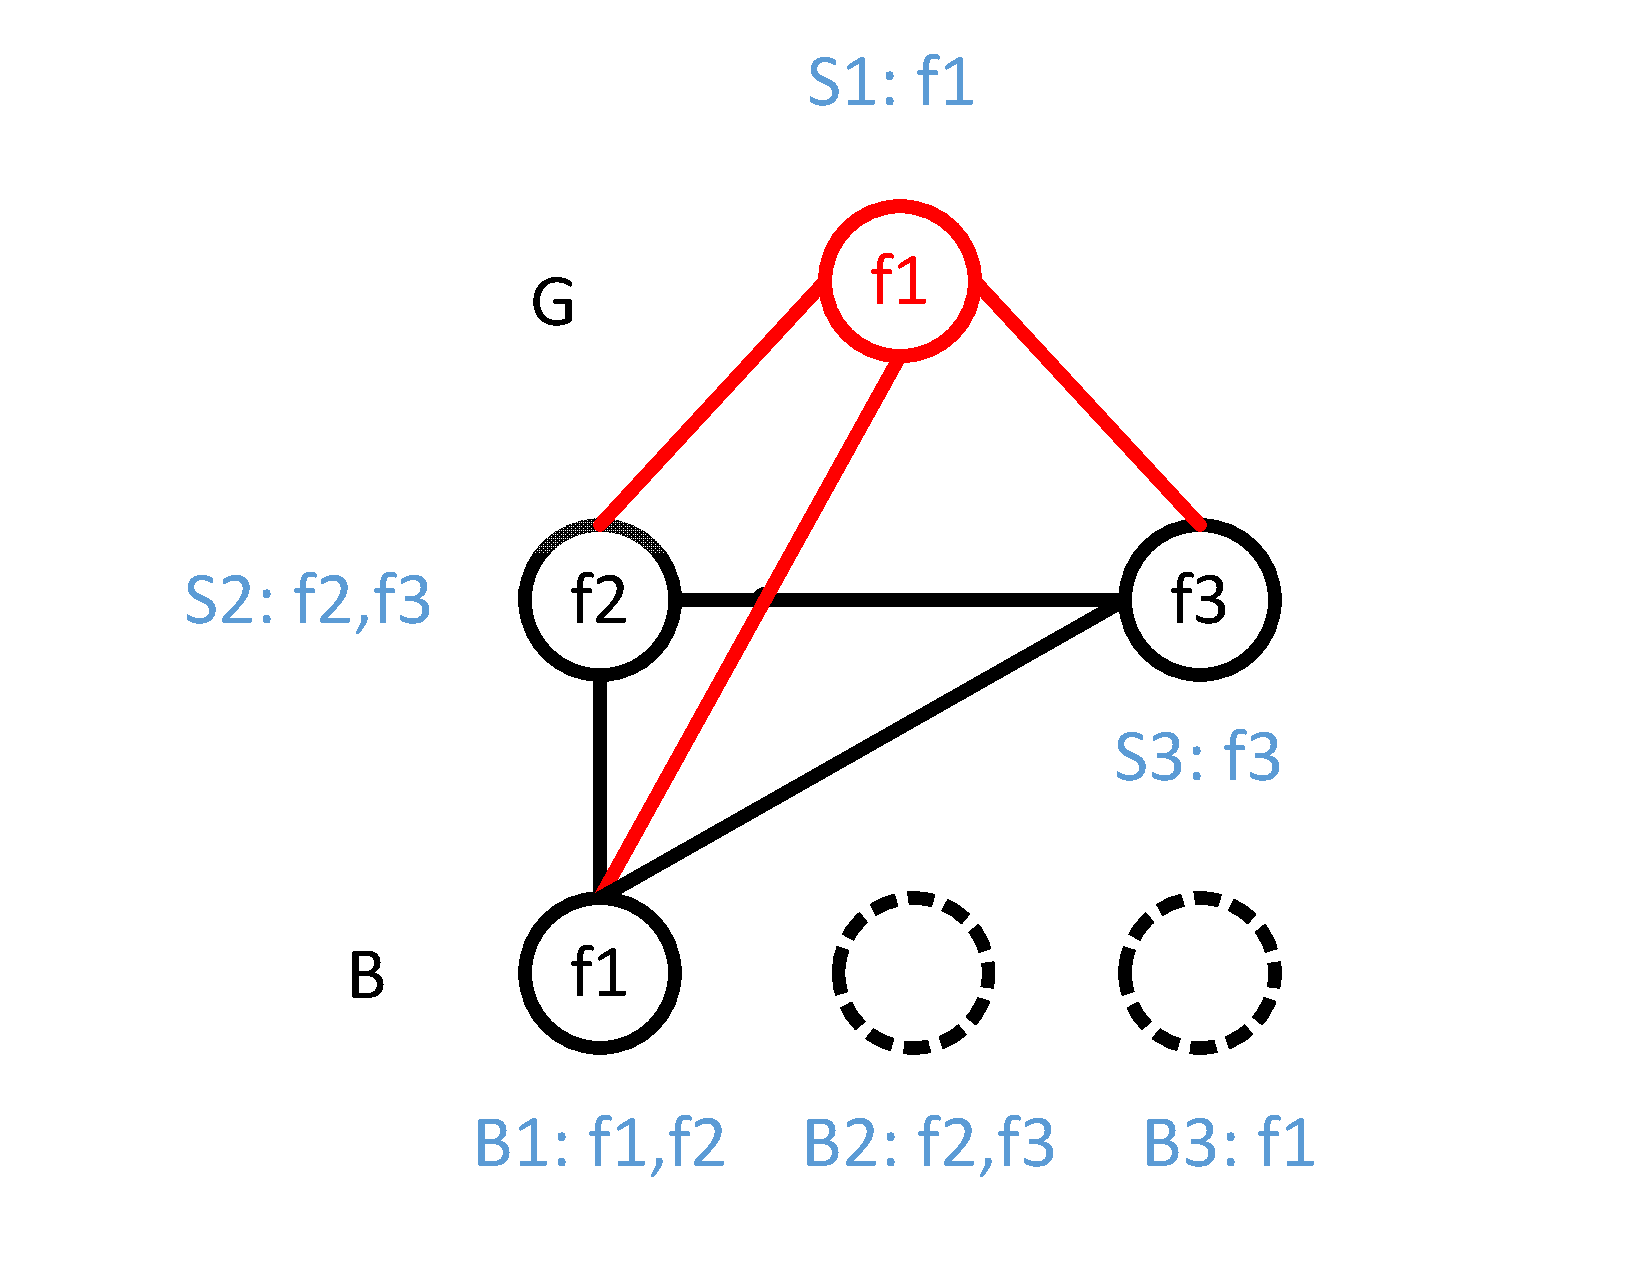
\includegraphics[width=1.5in]{Fig/SNFToptimal_n1Fail}\\
\caption{optimal $k$-FNFT($G(V,E,S),B(V,S)$) when node $v_1$ fail, node $v_1$ transform to $b_1$}\label{fig:SNFToptimal_n1Fail}
\end{minipage}
\hfill
\begin{minipage}[t]{0.3\linewidth}
\centering
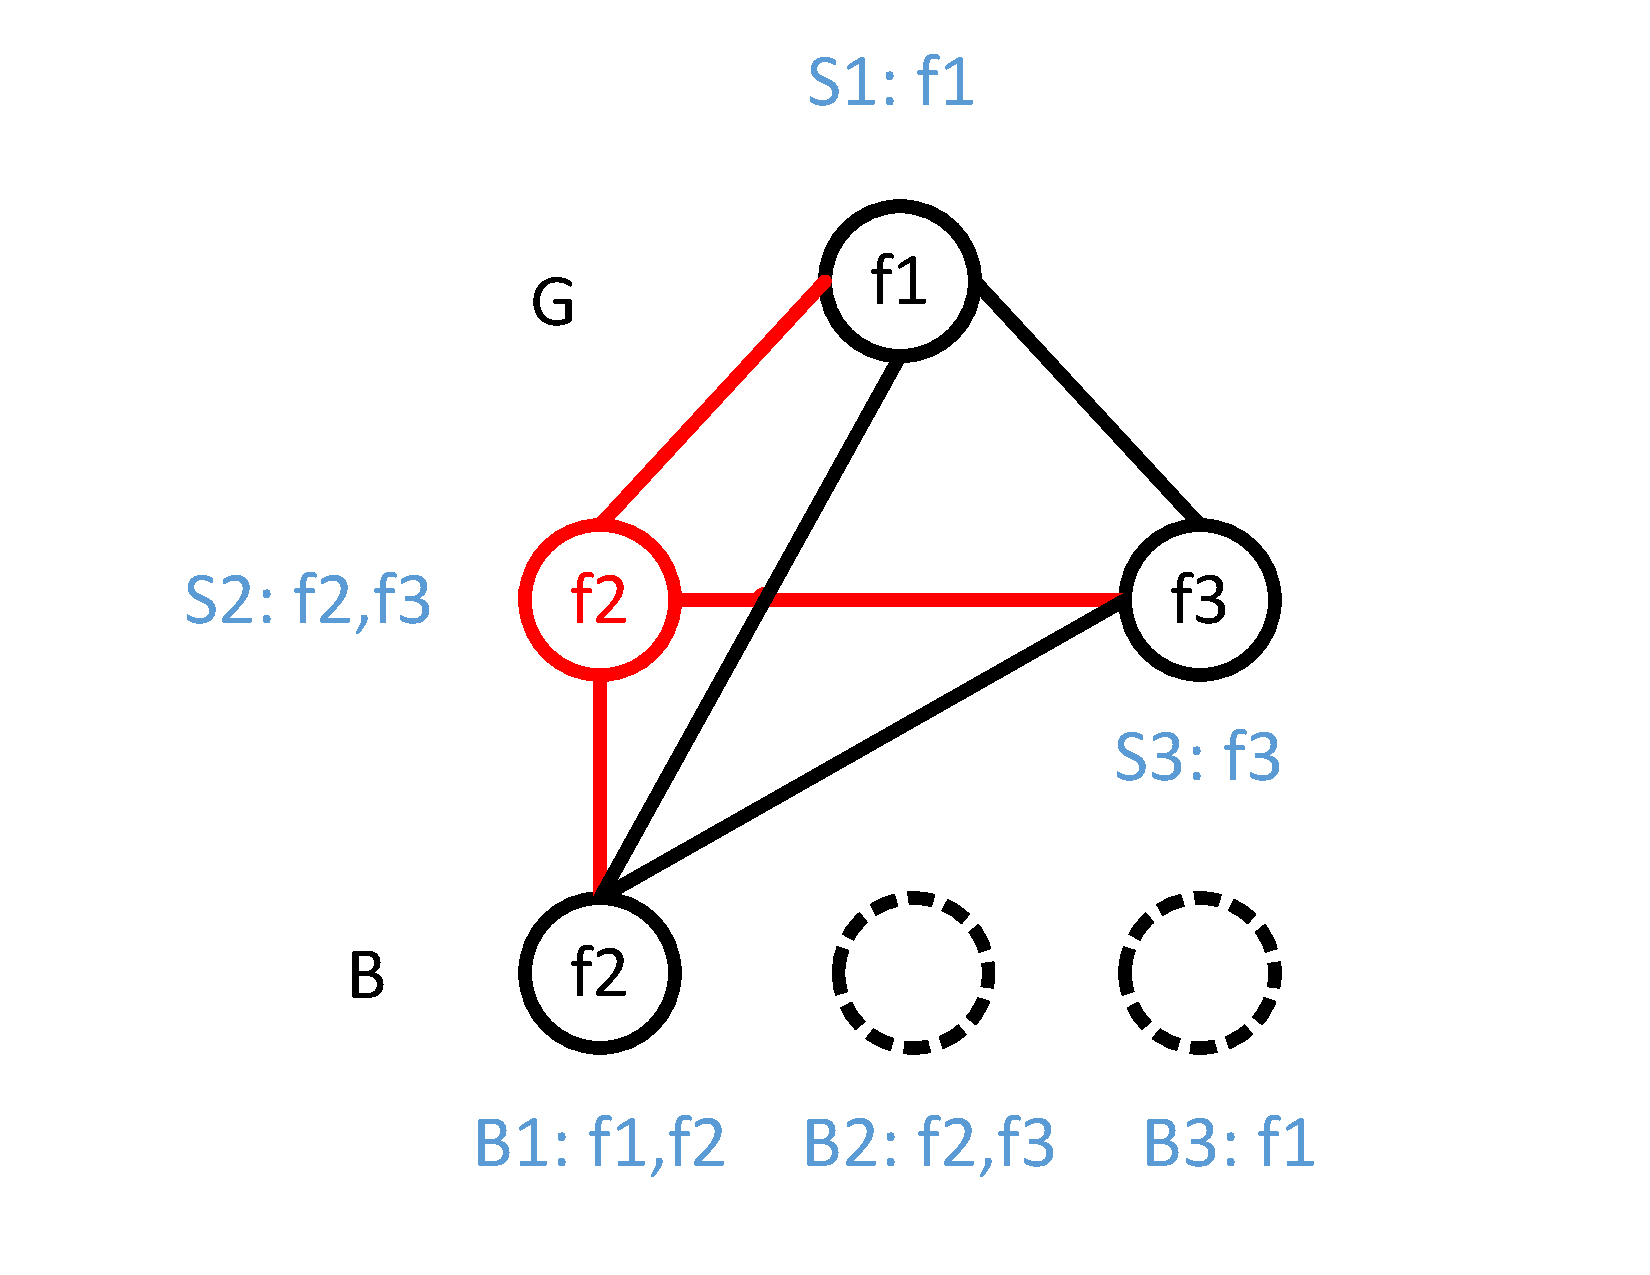
\includegraphics[width=1.5in]{Fig/SNFToptimal_n2Fail}\\
\caption{optimal $k$-FNFT($G(V,E,S),B(V,S)$) node $v_2$ fail, node $v_2$ transform to $b_1$}\label{fig:SNFToptimal_n2Fail}
\end{minipage}
\hfill
\begin{minipage}[t]{0.3\linewidth}
\centering
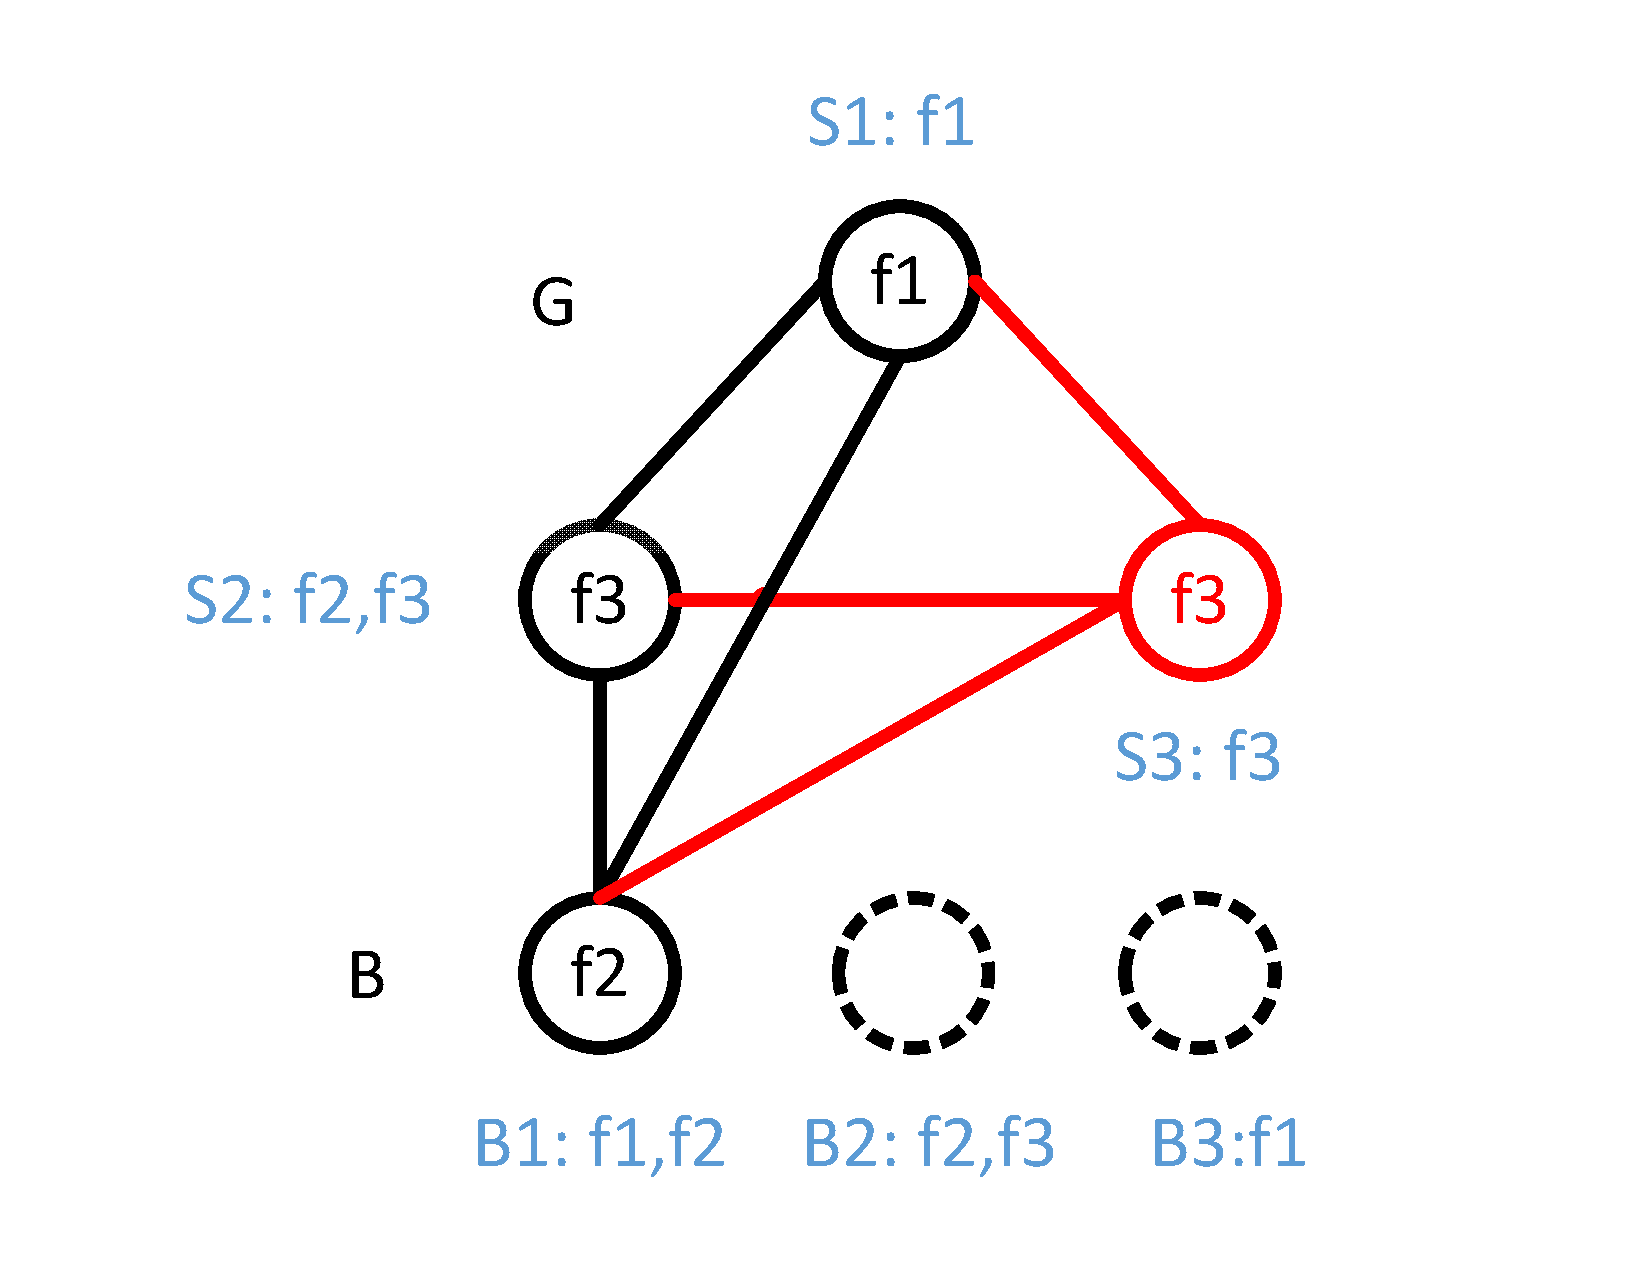
\includegraphics[width=1.5in]{Fig/SNFToptimal_n3Fail}\\
\caption{optimal $k$-FNFT($G(V,E,S),B(V,S)$) node $v_3$ fail, node $v_2$ transform to $b_1$, node $v_3$ transform to $v_2$}\label{fig:SNFToptimal_n3Fail}
\end{minipage}
\end{figure*}

\subsection{Complexity of Function Node Fault tolerant}
\label{sec:Complexity}
This computation complexity of $k$-FNFT graph problem $k$-FNFT($G(V,E,S)$) is NP, whose proof is described as below. when just exist one function type in Graph $G$, the problem is degenerated into k-node fault-tolerant graph problem. when Graph $G$ just have one type of function, we must add k backup node and add some edges into graph $G$ to construct $k$-FNFT graph, meantime the degenerated problem is of equivalency to k-node fault-tolerant $k$-NFT graph problem , which had been proofed as NP problem\cite{harary1996node}.

when added node set is given and confirmed aforehand , $k$-FNFT($G(V,E,S)$) is subproblem of the problem $k$-FNFT($G(V,E,S),B(V,S)$). Therefore, according to  the  reducibility theorem\cite{cormen2009introduction} in computer complexity field, it is easy to conclude that problem $k$-FNFT($G(V,E,S),B(V,S)$) is NP problem also.

The inter-inclusion relationship of the three problem is $k$-FNFT($G(V,E)$)$\subset$$k$-FNFT($G(V,E,S)$)$\subset$$k$-FNFT($G(V,E,S),B(V,S)$).

%Suppose topological structure of graph $G$ is path $P$, k-FNFT($P(V,E,S),B(V,S)$) is NP, the proof is below, exist one node $v_i(v_i\in V)$ and we add backup nodes and some edges to protect the node $v_i$, the former graph $P$ firstly is changed into $P+n$, nevertheless topological structure of $P+n$ may is not path, or be tree and non-tree graph. then protect other nodes of $V$ except node $v_i$, the problem become $(k-1)$-NFT problem.



However, this poses a limitation since the result only guarantees graph isomorphism and not equality without considering constraints of computation and communication. In other words, there may be a need to physically swap remaining VMs while recovering from some failure in order to return to the original infrastructure G. Recovery may then be delayed, or require more resources for such swapping operations.

%the computation complexity of k-FNFT($T(V,E,S),B(V,S)$) is similarly available.

%Edge fault tolerant problem is subgraph of node fault tolerant problem.
